\documentclass[11pt]{report}

% Paquetes y configuraciones adicionales
\usepackage{graphicx}
\usepackage[export]{adjustbox}
\usepackage{caption}
\usepackage{float}
\usepackage{titlesec}
\usepackage{geometry}
\usepackage[hidelinks]{hyperref}
\usepackage{titling}
\usepackage{titlesec}
\usepackage{parskip}
\usepackage{wasysym}
\usepackage{tikzsymbols}
\usepackage{fancyvrb}
\usepackage{xurl}
\usepackage{hyperref}
\usepackage{listings}
\usepackage{xcolor}
\usepackage{subcaption}
\usepackage[spanish]{babel}

\newcommand{\subtitle}[1]{
  \posttitle{
    \par\end{center}
    \begin{center}\large#1\end{center}
    \vskip0.5em}
}

% Configura los márgenes
\geometry{
  left=2cm,   % Ajusta este valor al margen izquierdo deseado
  right=2cm,  % Ajusta este valor al margen derecho deseado
  top=3cm,
  bottom=3cm,
}

% Configuración de los títulos de las secciones
\titlespacing{\section}{0pt}{\parskip}{\parskip}
\titlespacing{\subsection}{0pt}{\parskip}{\parskip}
\titlespacing{\subsubsection}{0pt}{\parskip}{\parskip}

% Redefinir el formato de los capítulos y añadir un punto después del número
\makeatletter
\renewcommand{\@makechapterhead}[1]{%
  \vspace*{0\p@} % Ajusta este valor para el espaciado deseado antes del título del capítulo
  {\parindent \z@ \raggedright \normalfont
    \ifnum \c@secnumdepth >\m@ne
        \huge\bfseries \thechapter.\ % Añade un punto después del número
    \fi
    \interlinepenalty\@M
    #1\par\nobreak
    \vspace{10pt} % Ajusta este valor para el espacio deseado después del título del capítulo
  }}
\makeatother

% Configura para que cada \chapter no comience en una pagina nueva
\makeatletter
\renewcommand\chapter{\@startsection{chapter}{0}{\z@}%
    {-3.5ex \@plus -1ex \@minus -.2ex}%
    {2.3ex \@plus.2ex}%
    {\normalfont\Large\bfseries}}
\makeatother

% Configurar los colores para el código
\definecolor{codegreen}{rgb}{0,0.6,0}
\definecolor{codegray}{rgb}{0.5,0.5,0.5}
\definecolor{codepurple}{rgb}{0.58,0,0.82}
\definecolor{backcolour}{rgb}{0.95,0.95,0.92}

% Configurar el estilo para el código
\lstdefinestyle{mystyle}{
  backgroundcolor=\color{backcolour},   
  commentstyle=\color{codegreen},
  keywordstyle=\color{magenta},
  numberstyle=\tiny\color{codegray},
  stringstyle=\color{codepurple},
  basicstyle=\ttfamily\footnotesize,
  breakatwhitespace=false,         
  breaklines=true,                 
  captionpos=b,                    
  keepspaces=true,                 
  numbers=left,                    
  numbersep=5pt,                  
  showspaces=false,                
  showstringspaces=false,
  showtabs=false,                  
  tabsize=2
}

\begin{document}

% Portada del informe
\title{Práctica 06. API Rest en Flask}
\subtitle{Administracion y Diseño de Bases de Datos}
\author{Cheuk Kelly Ng Pante (alu0101364544@ull.edu.es)}
\date{\today}

\maketitle

\pagestyle{empty} % Desactiva la numeración de página para el índice

% Índice
\tableofcontents

% Nueva página
\cleardoublepage

\pagestyle{plain} % Vuelve a activar la numeración de página
\setcounter{page}{1} % Reinicia el contador de página a 1

% Secciones del informe
% Capitulo 1
\chapter{Introducción}
La API RESTful es una interfaz que dos sistemas de computación utilizan para intercambiar información de
manera segura a través de Internet. La mayoría de las aplicaciones para empresas deben comunicarse con otras
aplicaciones internas o de terceros para llevar a cabo varias tareas

Flask es un framework para desarrollo web escrito en Python. Se puede utilizar para diversos tipos de
aplicación, entre ellas, desarrollo de APIs. Existen muchas maneras de implementar un API REST en Flask.
Desde usar el framework con lo que ofrece de base, o con la ayuda de extensiones con diferentes
configuraciones.

% Capitulo 2
\chapter{Actividad 1}
% 2.1
\section{Instalación del framework \emph{Flask} y la biblioteca \emph{psycopg2-binary}}
Para la instalación de \emph{Flask} y \emph{psycopg2-binary}, así como el desarrollo de la práctica
se va a crear un entorno virtual con \emph{virtualenv}. Primero se crea un directorio para el entorno
virtual y se accede a él.
\begin{verbatim}
$ mkdir practica_flask
$ cd practica_flask
\end{verbatim}

Dentro del directorio se crea el entorno virtual con \emph{virtualenv} y se instalará \emph{Flask} y
\emph{psycopg2-binary} dentro de él. Para ello, se ejecutarán los siguientes comandos:
\begin{verbatim}
$ sudo apt install python3.10-venv
$ python3 -m venv venv
$ . venv/bin/activate
$ pip install Flask
$ pip install psycopg2-binary
\end{verbatim}
\begin{figure}[H]
  \centering
  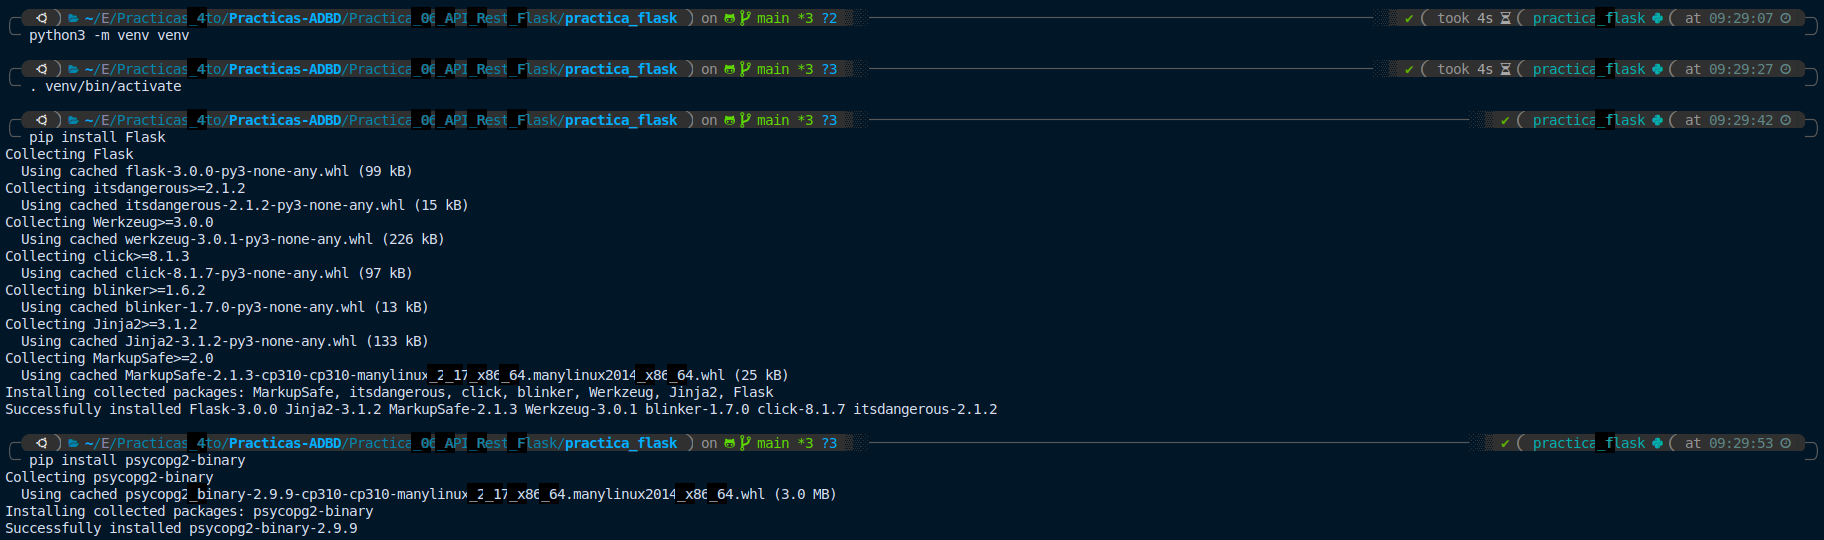
\includegraphics[scale=0.27]{img/instalation.png}
  \caption{Instalación de Flask y psycopg2-binary}
  \label{fig:instalacion_flask}
\end{figure}

% Nueva página
\cleardoublepage
\section{Despliegue de la aplicación web}
Para desplegar la aplicación web se va a crea una base de datos en \emph{PostgreSQL} con el nombre
de \emph{flask\_db}. Para ello, ejecutamos dentro psql el siguiente comando:
\begin{verbatim}
postgres=# CREATE DATABASE flask_db;
\end{verbatim}

Una vez creada la base de datos, sobre el directorio \emph{practica\_flask} se ponen los archivos que se van
a utilizar para el desarrollo de la práctica. Estos archivos son: \emph{app.py} e \emph{init.py} y dentro de
estos ficheros añadimos el usuario y contraseña de \emph{postgres} para poder acceder a la base de datos.

Ya modificados los archivos, se ejecuta el siguiente comando para desplegar la aplicación web:
\begin{verbatim}
$ python3 app.py
\end{verbatim}

Tambi\'en se puede ejecutar el siguiente comando para desplegar la aplicación web:
\begin{verbatim}
$ flask --app app.py run --host 0.0.0.0 --port=8080
\end{verbatim}

Con los comandos anteriores desplegamos la aplicación en local en el puerto 5000, pero va a
fallar ya que antes necesita la inicialización de la base de datos, lo cual se hace con el
siguiente comando:
\begin{verbatim}
$ python3 init_db.py
\end{verbatim}

\section{Creación de la base de datos e inserción de datos}
La creación de la base de datos se hizo en el apartado anterior y la inserción de datos se crean en el
script \emph{init\_db.py}.

\section{Personalizar la referencia \emph{About}}
Para personalizar la referencia del about creamos un nuevo archivo html en el directorio
templates \emph{about.html} en donde añadimos los nombres y apellidos de los integrantes del
grupo. Luego modificamos \emph{base.html} y el fichero \emph{app.py} para poder acceder a la nueva
sección.

\begin{figure}[H]
  \centering
  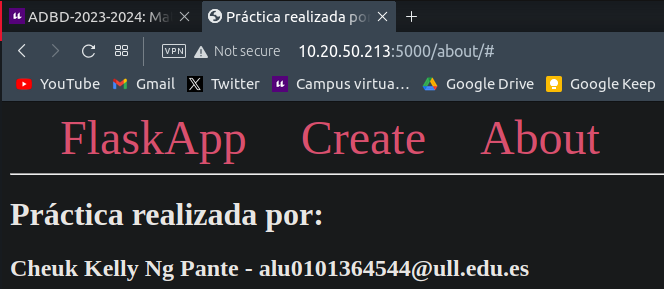
\includegraphics[scale=0.4]{img/about.png}
  \caption{About personalizado}
  \label{fig:about_personalizado}
\end{figure}

% Nueva página
\cleardoublepage

\section{Verificar funcionamiento de la operación de visualizar los registros}
Se puede verificar que se pueden visualizar los registros de la base de datos gracias a la función \emph{index()} que
se encuentra en el fichero \emph{app.py}, en el que se realiza la siguiente consulta para conseguir todas las entradas
de la tabla \emph{books}:
\lstset{style=mystyle}
\lstinputlisting[language=sql]{code/select_books.psql}

\begin{figure}[H]
  \centering
  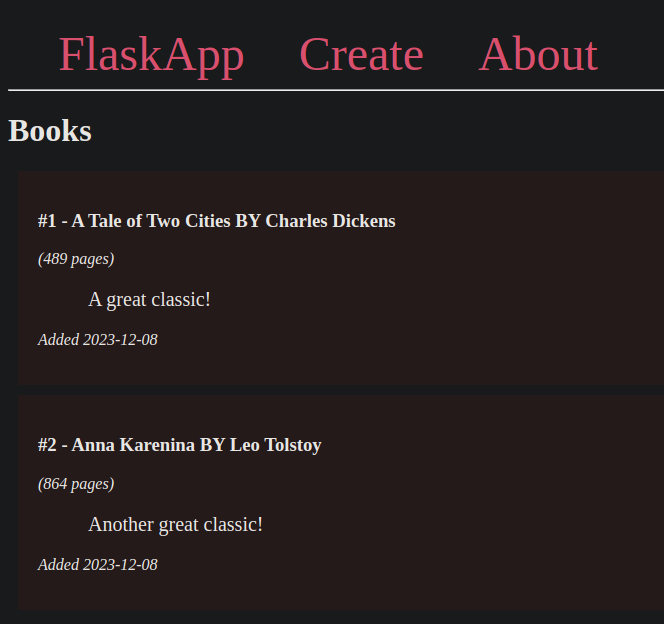
\includegraphics[scale=0.35]{img/visualizar_registros.png}
  \caption{Visualizar registros}
  \label{fig:visualizar_registros}
\end{figure}

% Nueva página
\cleardoublepage

\section{Verificar operacion de inserción de registros}
Se puede verificar que se pueden insertar registros en la base de datos gracias a la función \emph{create()} que
se encuentra en el fichero \emph{app.py}, en el que se realiza la siguiente consulta para insertar una entrada
en la tabla \emph{books}:
\lstset{style=mystyle}
\lstinputlisting[language=sql]{code/create_books.psql}

\begin{figure}[H]
  \centering
  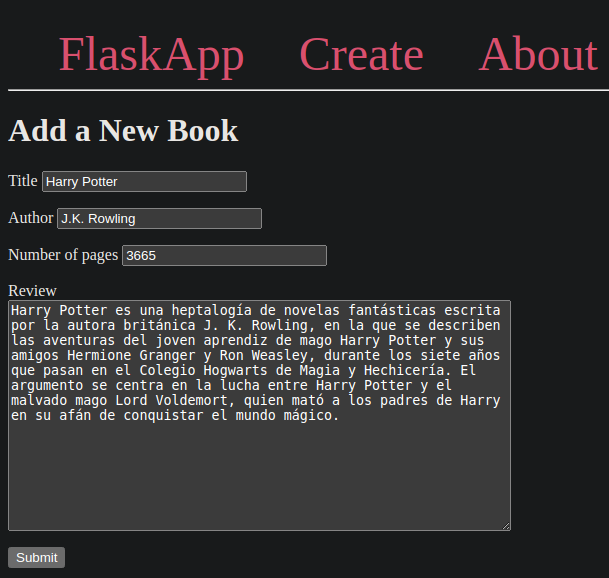
\includegraphics[scale=0.45]{img/create_book.png}
  \caption{Insertar registros}
\end{figure}

\begin{figure}[H]
  \centering
  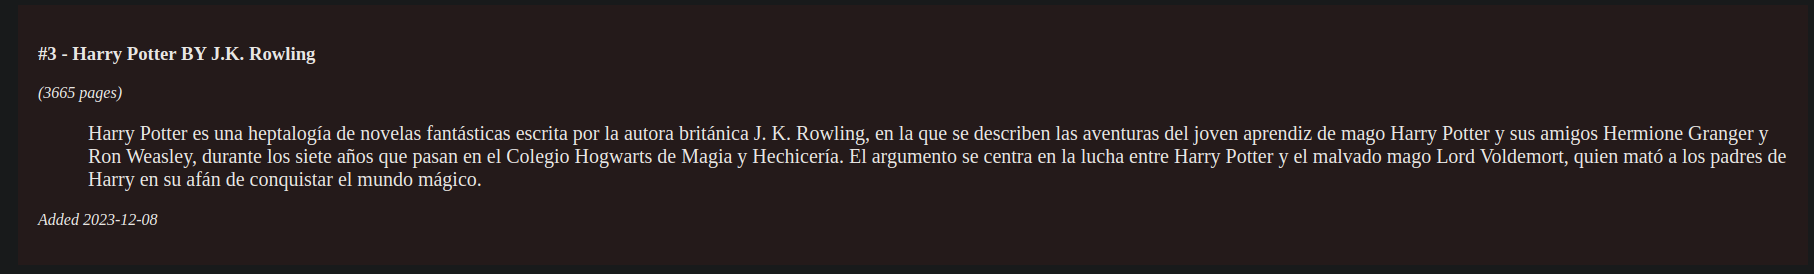
\includegraphics[scale=0.23]{img/added_book.png}
  \caption{Registro insertado}
\end{figure}

% Nueva página
\cleardoublepage

\section{Construcción de una REST API para la operación de borrado}
Para construir una REST API para la operación de borrado se crea una nueva función en el fichero \emph{app.py}
llamada \emph{delete()}, aqui el código en python:
\lstset{style=mystyle}
\lstinputlisting[language=sql]{code/delete_books.py}

Este código en python lo que hace es una consulta en sql para borrar una entrada de la tabla \emph{books},
aqui el código en sql:
\lstset{style=mystyle}
\lstinputlisting[language=sql]{code/delete_books.psql}

Además, hay que modificar el fichero \emph{base.html} para crear un apartado en el que se pueda borrar
un registro de la base de datos. Creamos fichero \emph{delete.html} en el directorio \emph{templates} y
lo codificamos para que se pueda borrar un registro de la base de datos con un formulario, aqui el código
en html:
\lstset{style=mystyle}
\lstinputlisting[language=html]{actividad_1/templates/delete.html}

\begin{figure}[H]
  \centering
  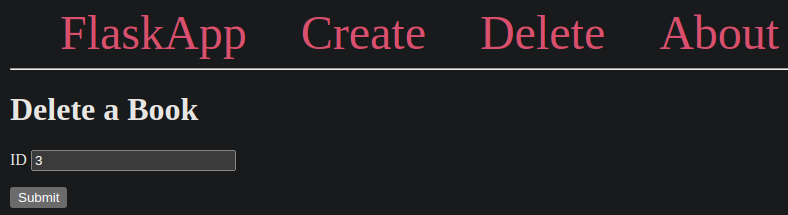
\includegraphics[scale=0.27]{img/delete_book.png}
  \caption{Borrar registros}
\end{figure}

\begin{figure}[H]
  \centering
  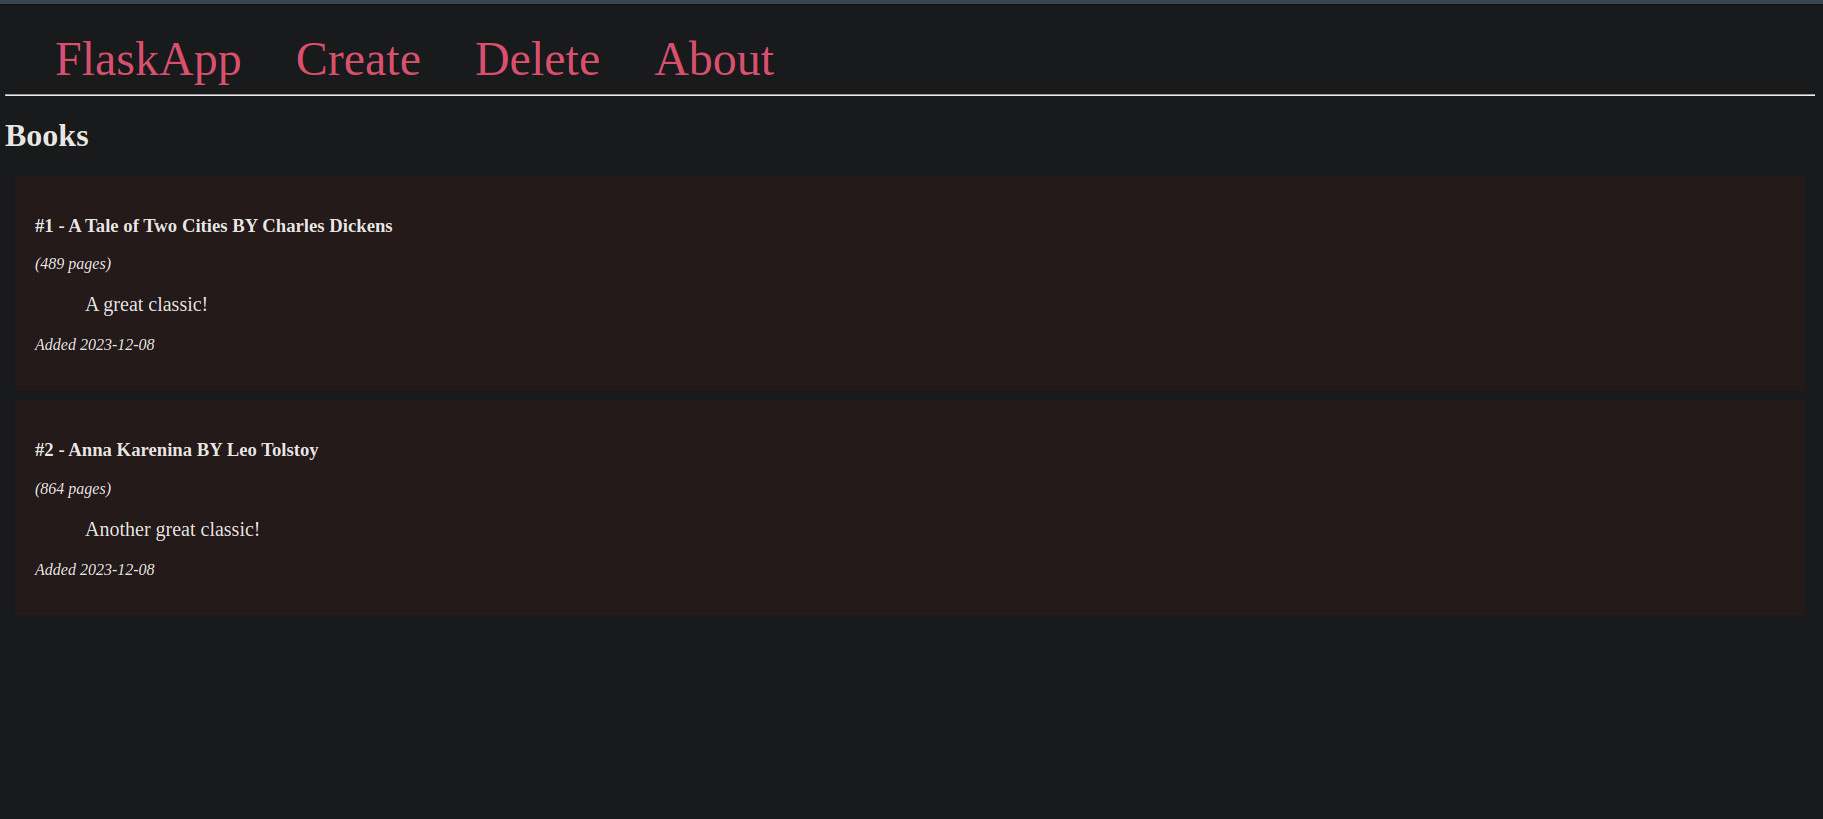
\includegraphics[scale=0.20]{img/book_already_deleted.png}
  \caption{Registro borrado}
\end{figure}

\section{Construcción de una REST API para la operación de actualización}
Para construir una REST API para la operación de actualización se crea una nueva función en el fichero \emph{app.py}
llamada \emph{update()}, en el que se actualizará un registro indicando su ID, aqui el código en python:
\lstset{style=mystyle}
\lstinputlisting[language=sql]{code/update_books.py}

Este código en python lo que hace es una consulta en sql para actualizar una entrada de la tabla \emph{books},
aqui el código en sql:
\lstset{style=mystyle}
\lstinputlisting[language=sql]{code/update_books.psql}

Luego, hay que modificar el fichero \emph{base.html} para crear un apartado en el que se pueda actualizar
un registro de la base de datos. Creamos fichero \emph{update.html} en el directorio \emph{templates} y
lo codificamos para que se pueda actualizar un registro de la base de datos con un formulario, aqui el código
en html:
\lstset{style=mystyle}
\lstinputlisting[language=html]{actividad_1/templates/update.html}

\begin{figure}[H]
  \centering
  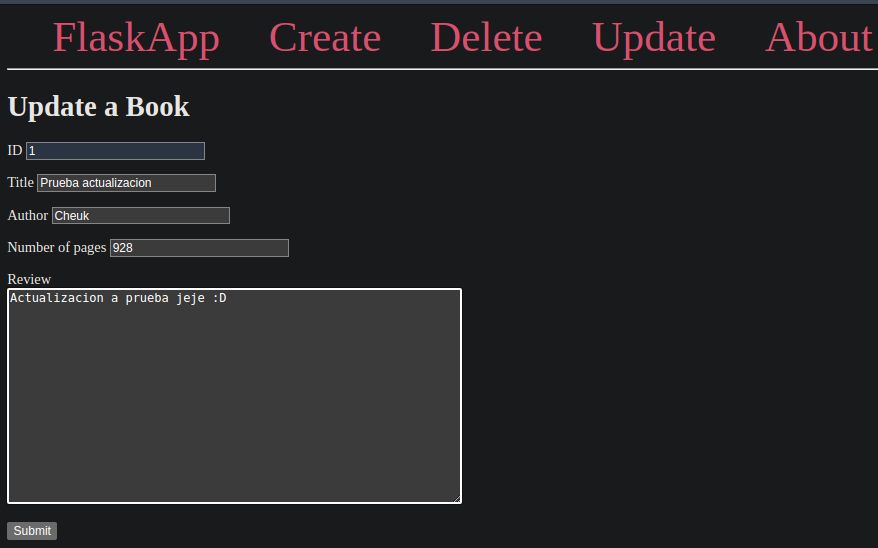
\includegraphics[scale=0.27]{img/update_book.png}
  \caption{Actualizar registros}
\end{figure}

\begin{figure}[H]
  \begin{subfigure}{0.5\textwidth}
    \centering
    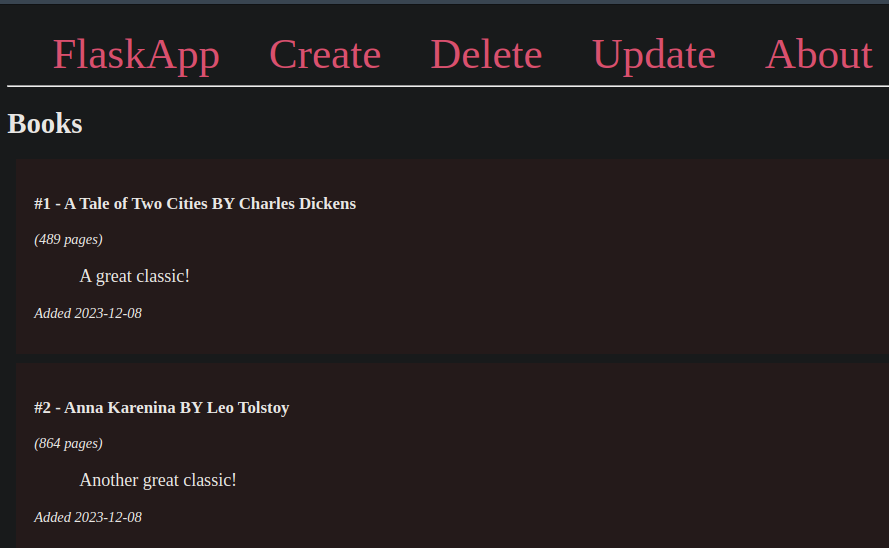
\includegraphics[scale=0.27]{img/non_update.png}
    \caption{Libro no actualizado}
  \end{subfigure}%
  \begin{subfigure}{0.5\textwidth}
    \centering
    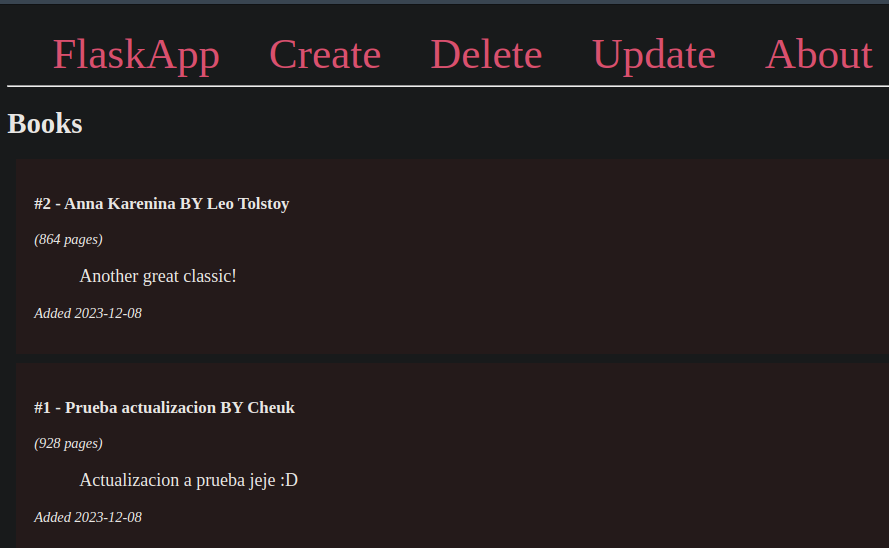
\includegraphics[scale=0.27]{img/updated_book.png}
    \caption{Libro actualizado}
  \end{subfigure}
  \caption{Actualización de registros}
\end{figure}

% Nueva página
\cleardoublepage

\chapter{Actividad 2}
\section{Desplegar la base de datos \emph{MyHome.psql}}
Para desplegar la base de datos a partir del script \emph{MyHome.sql} se ha utilizado el siguiente comando:
\begin{verbatim}
postgres=# \i MyHome.psql
\end{verbatim}

\begin{figure}[H]
  \centering
  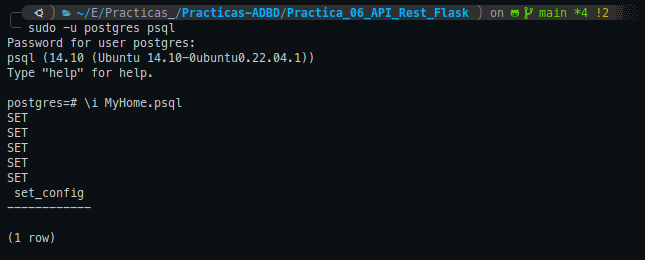
\includegraphics[scale=0.5]{img/myhome_script.png}
  \caption{Despliegue de la base de datos \emph{MyHome.psql}}
\end{figure}

\section{Construir con \emph{Flask} y \emph{psycopg2} las siguientes REST API}
Se va a crear un nuevo directorio de trabajo llamado \emph{actividad\_2} en el que tendrá las definiciones de la nueva
aplicación, las funcionalidades estarán en el fichero \emph{room\_app.py}.

\subsection{Retorno de la temperatura media de todas las habitaciones}
Para retornar la temperatura media de todas las habitaciones se crea una nueva función en el fichero \emph{room\_app.py}
llamada \emph{get\_avg\_temperature()}, en el que se retornará la temperatura media de todas las habitaciones, aqui el
código en python:
\lstset{style=mystyle}
\lstinputlisting[language=sql]{code/avg_temperature.py}

Lo que hace este código en python es una consulta en sql para obtener la temperatura media de todas las habitaciones,
\lstset{style=mystyle}
\lstinputlisting[language=sql]{code/avg_temperature.psql}

Luego, hay que modificar el fichero \emph{base.html} para crear un apartado en el que se pueda obtener la temperatura
media de todas las habitaciones. Creamos fichero \emph{average.html} en el directorio \emph{templates} y
lo codificamos para que se pueda obtener la temperatura media de todas las habitaciones, aqui el código en html:
\lstset{style=mystyle}
\lstinputlisting[language=html]{actividad_2/templates/average.html}

\begin{figure}[H]
  \centering
  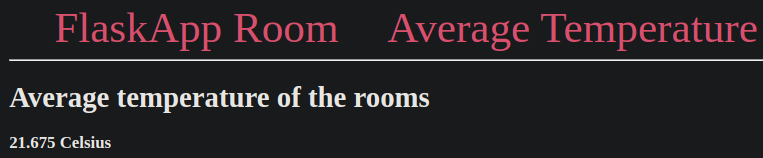
\includegraphics[scale=0.45]{img/average_temperature.png}
  \caption{Temperatura media de todas las habitaciones}
\end{figure}

\subsection{Retorno de la temperatura máxima de una habitación}
En este apartado se va a retornar la temperatura máxima de una habitación, para ello se hará lo mismo que en el apartado
anterior pero en la consulta extraeremos la temperatura máxima de una habitación, aqui el código en SQL:
\lstset{style=mystyle}
\lstinputlisting[language=sql]{code/max_temperature.psql}

\end{document}